% === CHAPTER 6: High-Level and Low-Level Design ===
\chapter{System Design and Architecture}

This chapter details the high-level and low-level architectural design of the KisaanMadad integrated mobile decision-support system. The architectural representations illustrate the structural organization, sub-system interactions, and data flows essential to fulfilling the project's functional and non-functional requirements. By delineating the overarching system architecture alongside the specific domain models and design tactics, this chapter provides the blueprint guiding the technical implementation of the platform.

\section{System Overview}
The KisaanMadad platform is structured as a robust client-server architecture tailored for resource-constrained environments in Punjab, Pakistan. The frontend constitutes a cross-platform Flutter mobile application designed to accommodate devices with limited processing power. This mobile client interfaces asynchronously with a central backend API powered by FastAPI (Python), which serves as the primary orchestration layer. The backend manages local data persistence through a PostgreSQL relational database and securely brokers external requests to third-party data providers, notably the NASA POWER API for meteorological coordinates and PAMRA/AMIS for localized commodity pricing data. The overarching objective of this architecture is to minimize bandwidth consumption while ensuring high availability of agricultural predictive models on the edge.

\section{Design Considerations}

\subsection{Assumptions and Dependencies}
\begin{itemize}
    \item \textbf{Connectivity Dependency:} The system assumes that while the farmer might operate in offline states, periodic connectivity is available to synchronize cached mandi datasets and synchronize the local FAO crop tables.
    \item \textbf{External API Stability:} Accurate irrigation modeling is strictly dependent on the continued availability and structural stability of the NASA POWER API endpoints.
    \item \textbf{Hardware Constraints:} The application design explicitly caters to low-memory Android devices common among smallholder farmers (i.e., devices with $<$ 2GB RAM), necessitating aggressive memory management.
\end{itemize}

\subsection{General Constraints}
\begin{itemize}
    \item \textbf{Limited Bandwidth:} Network payloads strictly consist of compressed JSON objects avoiding heavy graphical transmissions.
    \item \textbf{Multilingual Interfaces:} The software constraints require dynamic RTL (Right-to-Left) rendering capabilities to fully support the native Urdu typography cleanly.
    \item \textbf{Machine Learning Limitations:} Edge-based inferences using CNN-LSTM arrays must computationally complete within acceptable timeframes without draining the device's battery capacity.
\end{itemize}

\subsection{Goals and Guidelines}
\begin{itemize}
    \item \textbf{Offline-First Functionality:} Vital calculations (like the Hargreaves fallback routing and financial calculators) must trigger unhindered without active server connections.
    \item \textbf{Scalability:} The foundational FastAPI layer dictates that new ML models or updated FAO guidelines can be integrated smoothly without forcibly halting operations.
\end{itemize}

\section{System Architecture}
The system architecture physically partitions responsibilities into a classic three-tier arrangement: Presentation Tier (Mobile App), Logic Tier (Backend Services/ML Processing), and Data Tier (Database and External APIs). This segregation prevents monolithic dependencies.

\begin{figure}[htbp]
  \centering
  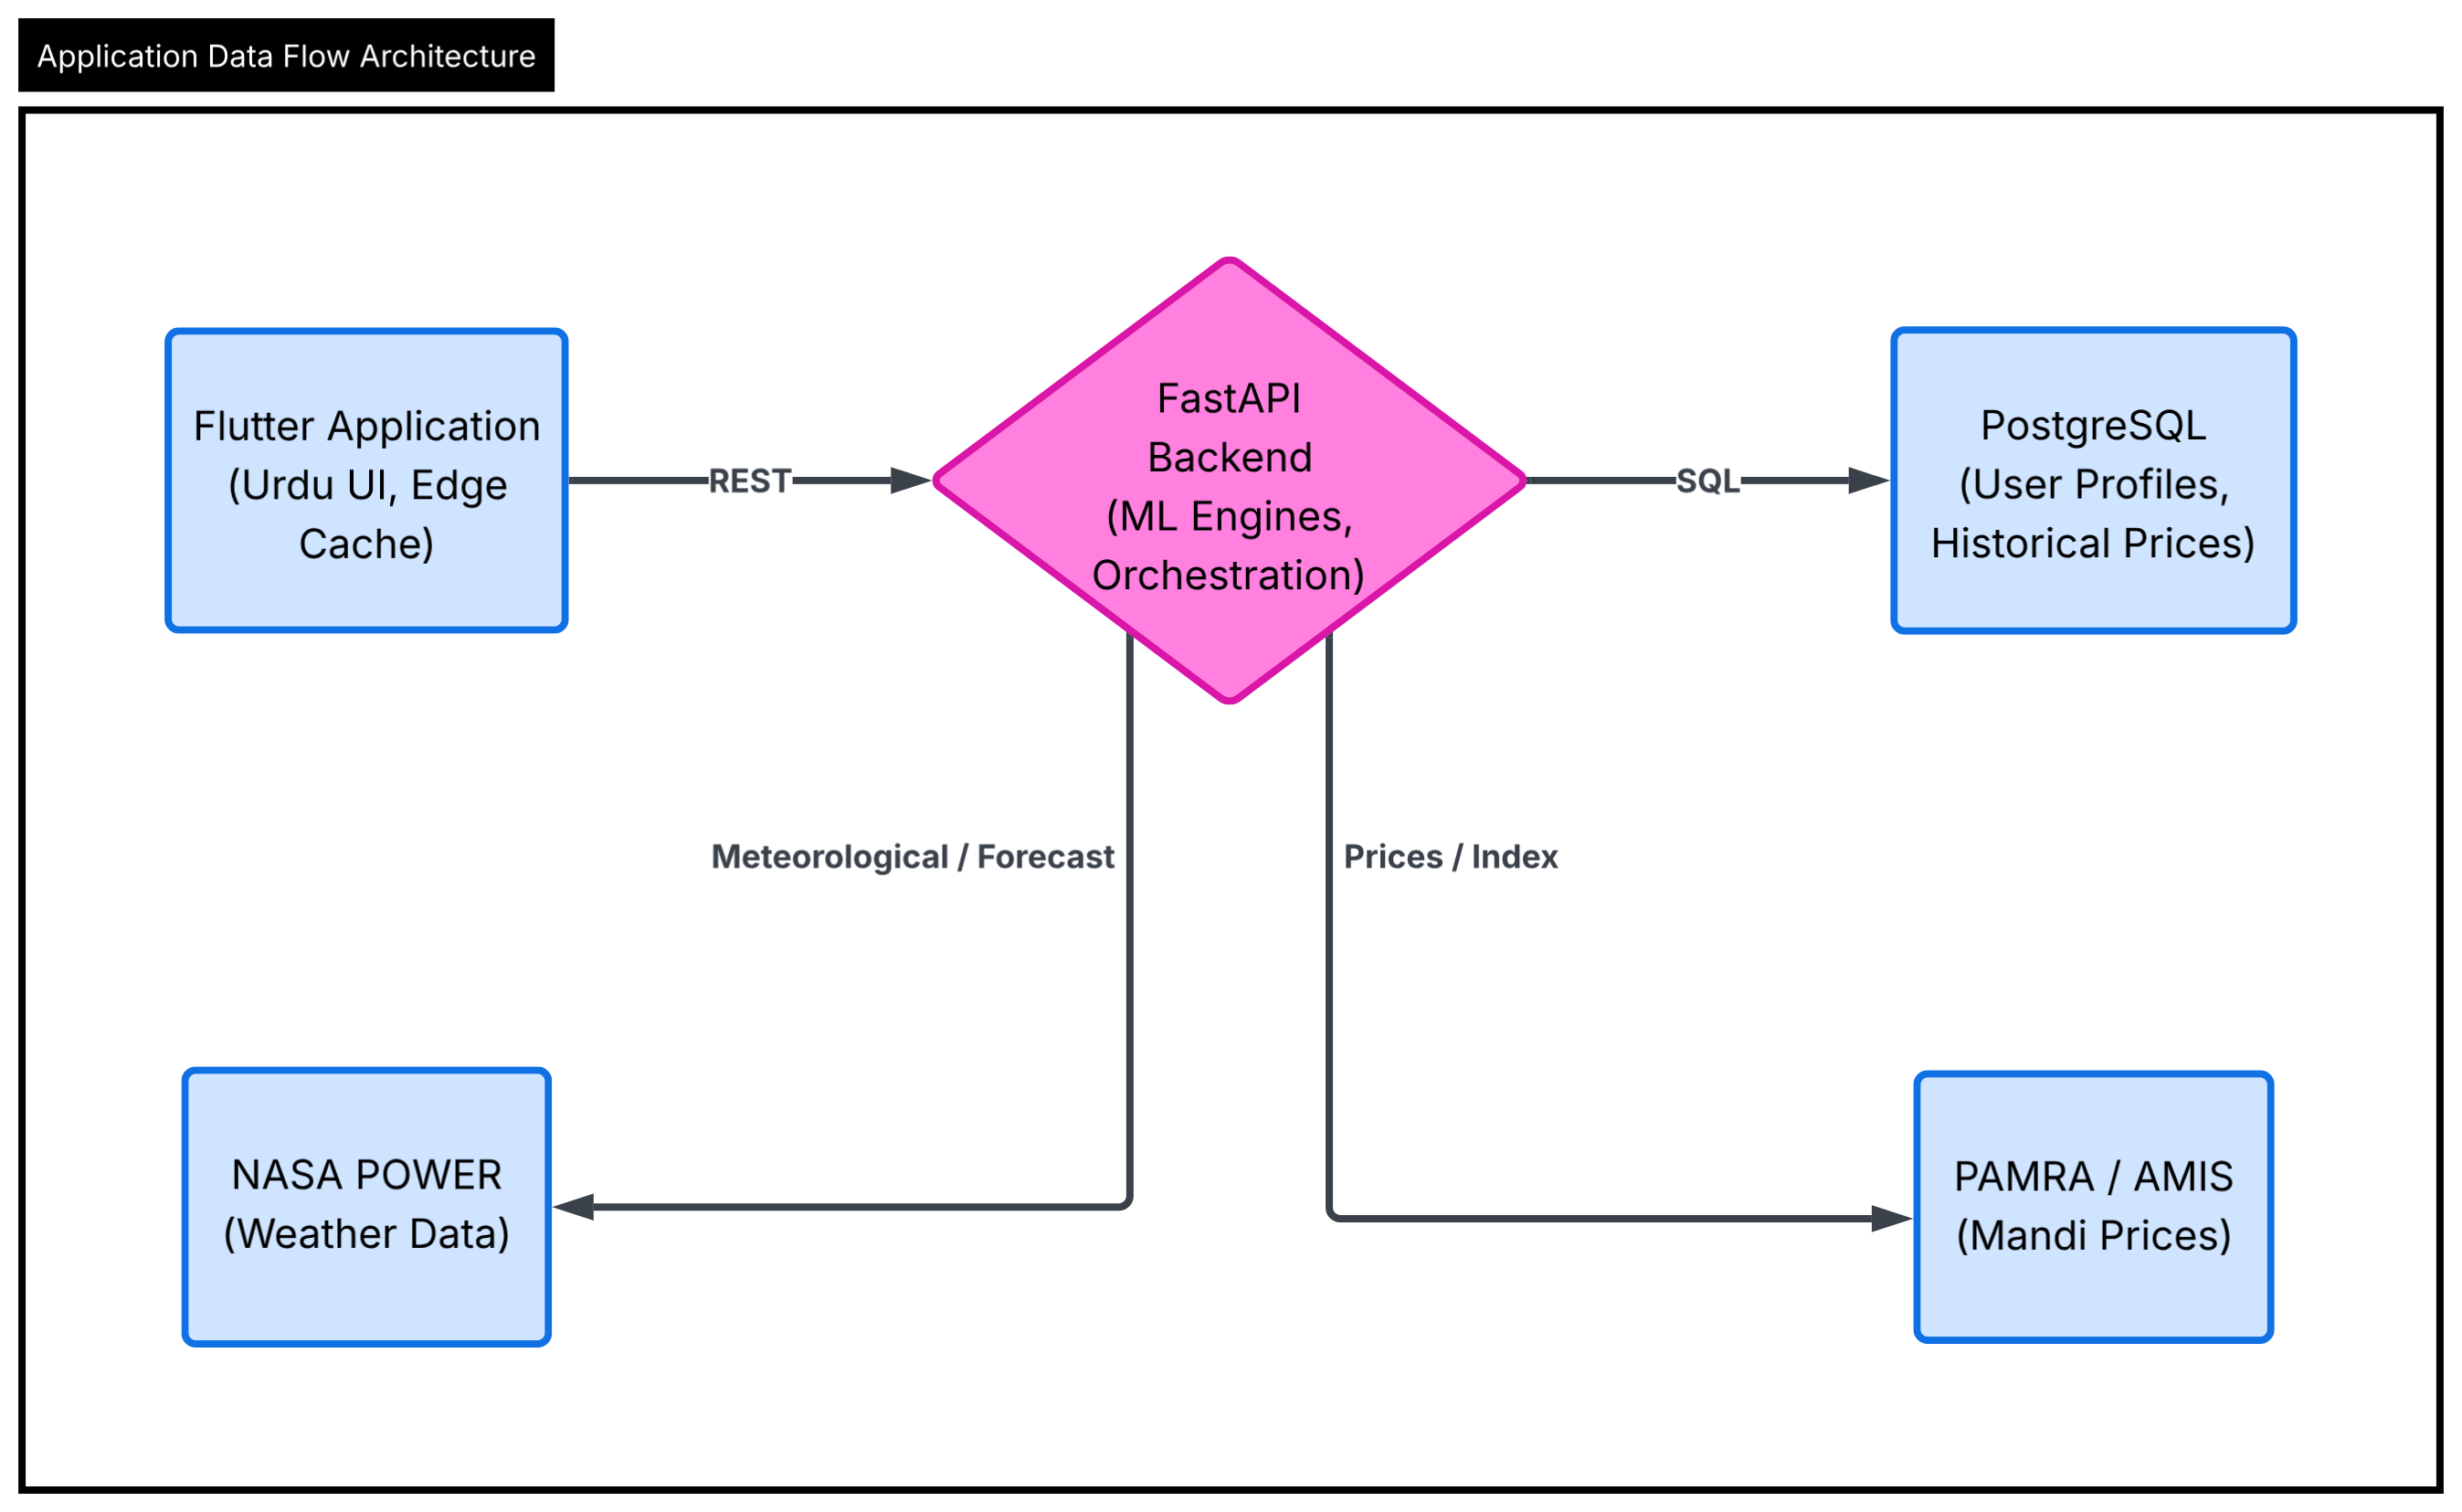
\includegraphics[width=\linewidth, keepaspectratio]{Figures/6.1.png}
  \caption{High-Level System Architecture of KisaanMadad.}
  \label{fig:high_level_arch}
\end{figure}

The diagram conceptually portrays the data transmission cycle. The Flutter application securely requests data parameters via RESTful principles directly to the FastAPI Backend. The server autonomously evaluates whether the request implies retrieving stable Postgres elements or necessitates real-time network interactions scaling to NASA POWER for evapotranspiration mechanics.

\subsection{Subsystem Architecture}
The central backend comprises four modular logical nodes reflecting the product scope. 
\begin{enumerate}
    \item \textbf{Price Forecasting Subsystem:} Ingests historical sequences, normalizes numerical tensors, and executes the CNN-LSTM predictor to output structured JSON confidence intervals.
    \item \textbf{Crop Recommendation Subsystem:} Houses the Multi-Criteria Decision Making matrix which cross-references incoming GPS latitudes alongside resident FAO calendars.
    \item \textbf{Irrigation Scheduling Subsystem:} Hosts the Penman-Monteith algorithms and Hargreaves fallback models executing strictly on retrieved atmospheric conditions.
    \item \textbf{Financial Planning Subsystem:} Operates as a purely deterministic mathematical orchestrator processing user-provided yield and loan parameters instantly.
\end{enumerate}

\begin{figure}[htbp]
  \centering
  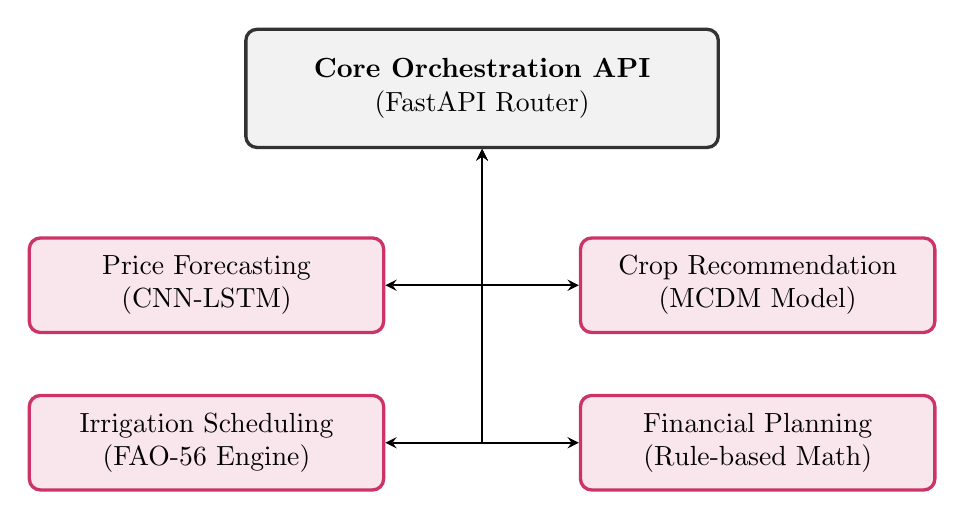
\begin{tikzpicture}[
      node distance=1.5cm,
      sub/.style={rectangle, draw=purple!80, fill=purple!10, very thick, minimum width=4.5cm, minimum height=1.2cm, align=center, rounded corners},
      main/.style={rectangle, draw=black!80, fill=gray!10, very thick, minimum width=6cm, minimum height=1.5cm, align=center, rounded corners},
      arrow/.style={<->, thick, >=stealth}
    ]
    
    \node[main] (core) at (0,0) {\textbf{Core Orchestration API} \\ (FastAPI Router)};
    
    \node[sub] (price) at (-3.5, -2.5) {Price Forecasting \\ (CNN-LSTM)};
    \node[sub] (crop)  at (3.5, -2.5) {Crop Recommendation \\ (MCDM Model)};
    \node[sub] (irrig) at (-3.5, -4.5) {Irrigation Scheduling \\ (FAO-56 Engine)};
    \node[sub] (fin)   at (3.5, -4.5) {Financial Planning \\ (Rule-based Math)};

    \draw[arrow] (core.south) |- (price.east);
    \draw[arrow] (core.south) |- (crop.west);
    \draw[arrow] (core.south) |- (irrig.east);
    \draw[arrow] (core.south) |- (fin.west);

  \end{tikzpicture}
  \vspace{0.5cm}
  \caption{Subsystem modular architecture detailing feature pathways.}
  \label{fig:subsystem_arch}
\end{figure}

\section{Architectural Strategies}

\subsection{Offline-First Mobile Caching}
This strategy addresses rural network instability. The mobile client implements an internal SQLite storage layer. Whenever network latency spikes or connections drop, localized mathematical requests naturally revert to the recent cached matrices. The system transparently flags stale data to the user using discreet UI indicators. 

\subsection{Graceful Degradation for Real-Time Models}
For the FAO-56 irrigation protocol, real-time meteorological failures risk pausing vital decisions. The architectural strategy strictly delegates computation. If precise NASA solar radiation streams falter, the backend algorithm intercepts the error and routes the process block toward the temperature-limited Hargreaves-Samani equation, structurally guaranteeing an actionable numeric output.

\section{Domain Model / Class Diagram}
The structural representation explicitly models the relationships defining the software environment. It clarifies associative multiplicity existing between the primary entity \textit{Farmer} and the underlying operational records.

\begin{figure}[htbp]
  \centering
  \begin{tikzpicture}[
      node distance=1.5cm and 2.5cm,
      class/.style={
        rectangle split,
        rectangle split parts=3,
        draw,
        very thick,
        minimum width=4cm,
        align=left,
        fill=white
      },
      arrow/.style={-{stealth}, thick}
    ]

    % Farmer Class
    \node[
        class,
        rectangle split part fill={black!10, white, white}
    ] (farmer) {
      \textbf{\hfil Farmer \hfil}
      \nodepart{two}
      - farmer\_id : UUID \\
      - name : String \\
      - phone : String \\
      - land\_size : Float
      \nodepart{three}
      + register() \\
      + syncData()
    };
    
    % Crop Class
    \node[
        class,
        rectangle split part fill={black!10, white, white},
        right=of farmer
    ] (crop) {
      \textbf{\hfil Crop \hfil}
      \nodepart{two}
      - crop\_id : Int \\
      - crop\_name : String \\
      - Kc\_value : Float \\
      - plant\_date : Date
      \nodepart{three}
      + fetchRecommend()
    };

    % MandiPrice Class
    \node[
        class,
        rectangle split part fill={black!10, white, white},
        below=of crop
    ] (price) {
      \textbf{\hfil MandiPrice \hfil}
      \nodepart{two}
      - price\_id : Int \\
      - avg\_price : Float \\
      - date : Date
      \nodepart{three}
      + runPrediction()
    };

    % Irrigation Class
    \node[
        class,
        rectangle split part fill={black!10, white, white},
        below=of farmer
    ] (irrig) {
      \textbf{\hfil IrrigationSchedule \hfil}
      \nodepart{two}
      - sched\_id : Int \\
      - ET0\_value : Float \\
      - status : Boolean
      \nodepart{three}
      + calcET0() \\
      + generateSchedule()
    };

    % Relationships
    \draw[arrow] (farmer.east) -- node[above, near start] {1} node[above, near end] {*} (crop.west);
    \draw[arrow] (crop.south) -- node[left, near start] {1} node[left, near end] {*} (price.north);
    \draw[arrow] (farmer.south) -- node[right, near start] {1} node[right, near end] {*} (irrig.north);

  \end{tikzpicture}
  \vspace{0.5cm}
  \caption{Domain Model / UML Class Diagram showing primary entity associations.}
  \label{fig:class_diagram}
\end{figure}


\section{Policies and Tactics}

\subsection{Asynchronous Executions}
Given the heavy computational burden associated with CNN-LSTM processing sequences, local predictive tactics forbid synchronous blocking operations. The application UI systematically initiates progress indicators corresponding to parallel thread executions, guaranteeing that visual presentation tiers never freeze during intense algorithm evaluations.

\subsection{Strict Dependency Injection}
The backend logic is rigorously encapsulated leveraging Dependency Injection (DI) paradigms. This structural tactic enforces that individual processing blocks (such as the API call to NASA POWER or database connection wrappers) exist completely decoupled. When deploying automated testing scripts during the QA phase, live dependencies are seamlessly replaced with localized mock arrays without restructuring underlying logic.

\section{Conclusion}
This chapter comprehensively detailed the overarching architecture managing KisaanMadad's execution matrices. The high-level deployment relies securely on asynchronous routing balancing a lightweight mobile client against sophisticated cloud operations. Deliberate structural fail-safes actively guarantee continuous decision-support capabilities despite severe environmental connectivity limits. The subsequent chapters will delineate the exact programmatic implementations and validation evaluations constructed upon these architectural blueprints.

% === END CHAPTER 6 ===
